% !TEX TS-program = xelatex
% !BIB TS-program = bibtex
\documentclass[12pt,letterpaper]{article}
\usepackage{style/dsc180reportstyle} % import dsc180reportstyle.sty

%%%%%%%%%%%%%%%%%%%%%%%%%%%%%%%%%%%%%%%%%%%%%%%%%%%%%%%%
%%%% Title and Authors
%%%%%%%%%%%%%%%%%%%%%%%%%%%%%%%%%%%%%%%%%%%%%%%%%%%%%%%%

\title{Evaluating Autonomous Drone Flight Robustness Under Environmental Disturbances Through NVIDIA Isaac Sim}

\author{Cheng-I Lin \\
  {\tt chl236@ucsd.edu} \\\And
  Po-Chen Lin \\
  {\tt p5lin@ucsd.edu} \\\And
  Colin Tran \\
  {\tt cot005@ucsd.edu} \\\And
  Haoshuo Bi \\
  {\tt hbi@ucsd.edu} \\\And
  Claire Tu \\
  {\tt c7tu@ucsd.edu} \\\And
  Mentor: Tauhidur Rahman \\
  {\tt trahman@ucsd.edu} \\} 

\begin{document}
\maketitle

%%%%%%%%%%%%%%%%%%%%%%%%%%%%%%%%%%%%%%%%%%%%%%%%%%%%%%%%
%%%% Abstract and Links
%%%%%%%%%%%%%%%%%%%%%%%%%%%%%%%%%%%%%%%%%%%%%%%%%%%%%%%%


\begin{abstract}
    \textcolor{LightGrey}{Modern autonomous drones navigate in various environments and encounter complex wind disturbances. Conventional control strategies such as proportional-derivative (PD) or Proportional-Integral-Derivative (PID) controllers may exhibit reduced tracking performance in such environments. Therefore, we investigate reinforcement learning algorithms that augment existing controls to stabilize the performance of quadcopters under wind disturbance and inspect their robustness under different simulations. We explore Proximal Policy Optimization (PPO) and Soft Actor-Critic (SAC) algorithms in our research. We attempt to conduct physics-based simulations to compare various types of existing flight control algorithms. Simulations are conducted in NVIDIA Isaac Sim, controlling a quadcopter to navigate its path in a simulated windy environment. The quadcopter would be tested in three types of simulated environments, including an empty grid, an indoor factory, and an outdoor environment. During our model training, we attempted a curriculum based training strategy that increases wind intensity and disturbance complexity. Preliminary experiments conducted by the team suggest that SAC-based residual controls reduce trajectory tracking error under windy conditions compared to PID-only controls. Future work would inspect other algorithms and focus on systematic comparisons among other algorithms. There is also potential to look into other types of weather conditions and how models can respond to them.}
\end{abstract}


\begin{center}
%Website: \url{https://abc.github.io/} \\
Code: \url{https://github.com/randonDsc/drone_final_project1}
\end{center}

\maketoc
\clearpage

%%%%%%%%%%%%%%%%%%%%%%%%%%%%%%%%%%%%%%%%%%%%%%%%%%%%%%%%
%%%% Main Contents
%%%%%%%%%%%%%%%%%%%%%%%%%%%%%%%%%%%%%%%%%%%%%%%%%%%%%%%%

\section{Introduction}
\subsection{Background \& Motivation}
Unmanned aerial vehicles (UAVs), commonly referred to as drones, have gained increasing importance in the technological world due to their abilities to operate in environments that are considered difficult, dangerous, or inefficient for humans. Through their autonomous mobility, environmental awareness, and precise navigation, drones have become the primary tool utilized for infrastructure inspection, search and rescue, environmental monitoring, and aerial data collection. Despite the advantages, drones suffer the same challenges of achieving reliable, stable, and efficient autonomous flights as all other aerial vehicles. Without human controls, drones are constantly under the influence of external disturbances such as adverse weather conditions and foreign object obstacles. For instance, wind can introduce uncertainty to the flight paths by changing the aerodynamics of airflow, directing translational and angular forces that obstruct the drone’s motions. Meanwhile, precipitation can interfere with the rotational power of the propeller blades and hinder sensory data used for capturing critical navigation data, negatively impacting the intended flight trajectory. These disturbances can consequently cause flight deviations, increased control effort, or loss of stability, especially during demanding navigation tasks. Therefore, understanding how environmental or other outside conditions influence drone performance is essential for improving the reliability and quality of autonomous aerial systems.

To approach this issue, we need to investigate a multitude of possible scenarios, including the disturbances a drone may encounter during its flight, the repercussions of each disturbance on the drone, and the possible solutions that can remedy or counteract these disturbances. Although it is difficult to gather well-rounded data in real life settings, we can accomplish this through physics based simulations, providing an accessible approach without the costs and safety risks associated with repeated physical flight experiments. In a simulated environment, we can directly manipulate wind conditions, configure flight scenarios, monitor internal drone states, and repeat experiments under controlled states, allowing the development of a comprehensive investigation. However, the effectiveness of computational simulations ultimately depends on the accuracy to which the simulations can reflect real world drone dynamics, aerodynamic disturbances, and sensor behaviors. Fortunately, many researchers, scientists, and other professionals have built functional simulation platforms for public access. NVIDIA Isaac Sim is one of those platforms, containing a wide scope of libraries for robotics simulation, testing, and synthetic data generation. Although there are other simulation applications such as MuJoCo, Isaac Sim offers photorealistic ray-traced rendering, high-fidelity perception sensor simulations, and massive synthetic data generation, allowing for more complex, detailed drone simulations. Therefore, our project mainly uses NVIDIA Isaac Sim to develop and evaluate drone simulation workflows, addressing the challenges of environmental adversities. We focus on reproducing environmental disturbances, observing their effects on drone behavior, and assessing whether conventional and learning based control strategies can maintain reliable flight across varied conditions. Ultimately, we seek to understand both how autonomous drones can better respond to environmental uncertainty and how simulation can support meaningful, robust evaluations of their performance.


\subsection{Literature Review \& Discussion of Prior Work}

Autonomous drone flight control has become an increasingly important field of research with the growing development and integration of drones in multiple settings, ranging from surveillance to delivery services to search and rescue operations. One of the biggest challenges of modern day autonomous drone flight is the maintained stability and accuracy of navigation against adverse weather conditions, particularly strong winds and precipitation. These external disturbances can affect a drone’s position, velocity, and orientation potentially steering the drone off of its original flight path. A lot of current research has focused on the application and use of reinforcement learning (RL), as well as other advanced control methods and algorithms to improve the ability of drone flight and its adaptability to different environmental conditions.

One important area of prior research has to deal with the development of realistic physics based environments/engines for training and evaluating autonomous drones and robots in general. In “Pegasus Simulator: An Isaac Sim Framework for Multiple Aerial Vehicles Simulation,” \cite{jacinto2024pegasus} introduced a simulation framework (Pegasus) built on NVIDIA’s Isaac Sim that allowed researchers to model multiple aerial vehicles in realistic environments, simulate onboard flight sensors, as well as integrate other existing flight control systems like the PX4. This research provided a useful middle ground between traditional robotics simulators and more complex game engine based environments like Unity. While simulators built on engines like Unity can be highly realistic, they have a steeper learning curve because of the nature of Unity being built specifically for game development. On the other hand, robotics simulators are easier to use for this purpose but lack the advanced rendering capabilities that game engines have. Pegasus bridges this gap by providing the realistic physics based environment with a framework and extension made for testing and simulating robotics. This allows researchers to focus more on developing and testing flight control algorithms rather than having to build these simulation environments from scratch. However, while Pegasus provides a realistic simulation environment for developing and testing autonomous flight-control algorithms, the research does not specifically investigate how drones can adapt to adverse environmental conditions such as wind disturbances.

Another area of research focused on the use of reinforcement learning as a method to improve existing flight controllers against wind disturbances. In “SAC-Assisted Hybrid Control for Quadrotor Path Following under Wind Disturbances,” \cite{heo2026sac} explored the usage of reinforcement learning alongside traditional flight control systems to see how well quadrotor drones can improve flight performance against adverse wind conditions. The researchers proposed a combined system using a conventional P-PD based quadrotor controller as well as a Soft Actor-Critic (SAC) controller (SAC is a reinforcement learning algorithm designed for continuous control tasks). Essentially, the traditional quadrotor controller was responsible for general flight stability but the SAC system also learned, via extended training, to make additional adjustments to the motor thrusts to compensate for external disturbances such as wind. The researchers evaluated this system using four different simulation scenarios: hovering, line-segment tracking, circular path following, and figure-eight path following. Their evaluations found that the SAC-assisted consistently improved positional accuracy compared to the baseline controller, more specifically it reduced the “three-dimensional position RMSE by 31.82\%, 13.15\%, 11.75\%, and 26.29\% in the four scenarios, respectively, compared with the baseline controller.” \citep{heo2026sac} Their results demonstrate that the usage of reinforcement learning can help improve the performance of existing flight controllers, specifically when we are dealing with environmental disturbances like wind, which conventional controllers may struggle to compensate for under changing environments and conditions.

In another similar paper, “Improving Wind Resistance Performance of Cascaded PID Controlled Quadcopters using Residual Reinforcement Learning,” \cite{ishihara2023wind} explored the usage of reinforcement learning to improve wind resistance of quadrotor flight controllers. Similarly to \cite{heo2026sac}, they proposed a hybrid control system including a traditional cascaded PID controller with an additional RL trained approach to compensate for any sort of wind disturbance. One major difference between this study and \cite{heo2026sac} was that the researchers not only evaluated the system’s performance in simulation, but also transferred the reinforcement learning controller to a physical quadcopter to test in real life environments. This allowed them to directly experiment in real life situations and they found that the proposed system could reduce positional deviations by approximately 50\% compared to the conventional basic cascaded PID controller \citep{ishihara2023wind}. These findings further support the use of reinforcement learning within our domain to improve drone flight robustness under increased environmental disturbance.


\subsection{Relevant Data}
Instead of researching and implementing existing observational datasets, our project primarily uses synthetic data generated through physics based drone simulations. This is well suited for our experimental objectives as we can directly supervise various environmental conditions and flight configurations through altering simulation parameters, repeatedly obtaining observations in a consistent, reproducible manner. Our simulations use representations of multirotor drone dynamics, primarily the Iris quadcopter model, including physical properties such as mass, inertia, rotor actuation, and the relationship between applied forces and resulting motion. This guides the data analytical processes by demonstrating how the drone is affected by environmental conditions during each simulation. Specifically, the environmental configurations and flight task definitions are programmed with variables such as mean wind speed and direction, gust intensity, temporal variation, turbulence strength, correlation times, and random seeds (to generate random values to distinguish between simulated samples).

In each simulation, we collected various quantitative and qualitative data. For time indexed flight state measurements, the collected data consist of three dimensional position, linear velocity, acceleration, orientation, angular velocity, and motor commands (four commands for four motors of a quadcopter). These statistics provide the basis for evaluating drone stability and trajectory tracking during each simulated timestamp, indicating where the drone is, how fast it is going, how well it can turn in curved paths, and what motors are responsible for each thrust pattern. Besides the internal measurements of the drone, we also equipped multiple advanced sensors and inertial measurement units (IMU) on the drone model to record external data. For simulated sensory outputs, the captured data consist of RGB and depth images and videos from a front-facing drone camera, rotational rates across three axes from a gyroscope, acceleration measurements from an accelerometer, and 3D point clouds from a Hesai XT32 LiDAR (Light Detection and Ranging). These readings provide the foundation for evaluating flight paths to reflect autonomous control inputs, exploiting sensory details to accurately determine locational coordinates and surrounding conditions. 

By collecting sensory data, we ensure an autonomous feedback loop where the drone can actively take in exterior inputs by itself, allowing it to respond to different changes of environmental conditions without any human interventions. Although using sensory data is the optimal practice in autonomous drone flights, we also collected ground truth data from the simulator platform so that we can know the exact position, velocity, and orientation of the drone without any sensor and calculation noise or error. Retaining ground truth data helps us validate simulated sensor measurements and provides the prototype iteration of the simulation where sensor feedbacks are not yet incorporated. These are all documented in the flight logs in the form of CSV files, which are associated with the corresponding environmental scenario, controller configuration, and simulation parameters.  

Flight logs will be used to support the calculation of quantitative performance metrics, including position root mean squared error (RMSE), cross-track deviation, maximum trajectory error, altitude error, flight completion, and failure frequency. Control related measurements, such as motor saturation, may provide additional insight into the physical effort required to counteract environmental disturbances. By collecting comparable measurements across repeated flight scenarios, we aim to characterize how changes in environmental conditions influence drone behavior and assess whether different control strategies provide measurable improvements.



%%%%%%%%%%%%%%%%%%%%%%%%%%%%%%%%%%%%%%%%%%%%%%%%%%%%%%%%
\iffalse
\section{Methods}

\section{Results}

\section{Discussion}

\section{Conclusion}

\section{\LaTeX{} Typesetting Examples}

{\color{blue} This is not a real section; it's just here to show examples of how to format various components. Remove it before submitting!}

\subsection{\LaTeX{} Basics}

Here's \textbf{bold} and \textit{italicized} text. Here's \texttt{text\_that\_looks.like(code)}.

\begin{itemize}
    \item Here's a regular bulleted list item.
    \item And another.
\end{itemize}

Here's a \href{https://datascience.ucsd.edu}{hyperlink}. If you want to use a numbered list, you can experiment with:

\begin{enumerate}
    \item This.
    \item This.
    \item And this.
\end{enumerate}

Here's how you might include a snippet of actual code:

\begin{verbatim}
# If you want to use syntax highlighting, look into the minted package.
def f(x):
    return 2 * x + 3
\end{verbatim}

Here's how you might format a single equation:

$$\int_{-\infty}^\infty f_X(x)dx = 1$$

And a chain of equations:

\begin{align*}
    \frac{1}{n}\sum_{i = 1}^n (x_i - \bar{x})^2 &= \frac{1}{n}\sum_{i = 1}^n (x_i^2 - 2x_i\bar{x} + \bar{x}^2)
    \\ &= \frac{1}{n}\sum_{i = 1}^n x_i^2 - \frac{2}{n}\bar{x}\sum_{i = 1}^n x_i + \frac{\bar{x}^2}{n}\sum_{i = 1}^n 1
    \\ &= \frac{1}{n}\sum_{i = 1}^n x_i^2 - 2\bar{x}^2 + \bar{x}^2
    \\ &= \frac{1}{n}\sum_{i = 1}^n x_i^2 - \bar{x}^2
\end{align*}


\subsection{Figure Examples}

Here are some example figures. 
Figure \ref{fig:somefig1} presents a scatter plot.

\begin{figure}[htbp]
\centering
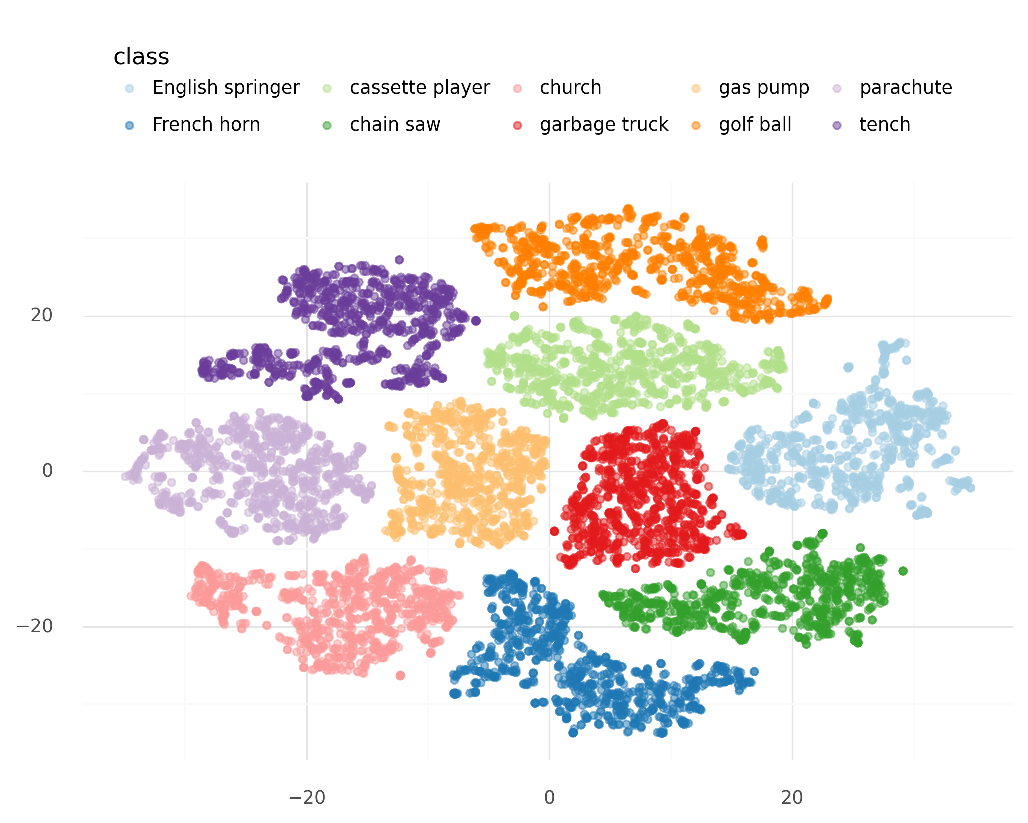
\includegraphics[width=.65\linewidth]{figure/somefig1.pdf}
\caption{Yes, put a few words or sentences here explaining what is in the figure.}
\label{fig:somefig1}
\end{figure}

Figure \ref{fig:someotherfigs} presents some summaries of the performance of our model.
The left panel of Figure \ref{fig:someotherfigs} presents something.
The right panel of Figure \ref{fig:someotherfigs} presents some other things.

\begin{figure}[htbp]
\begin{minipage}{0.53\linewidth}
  \centering
  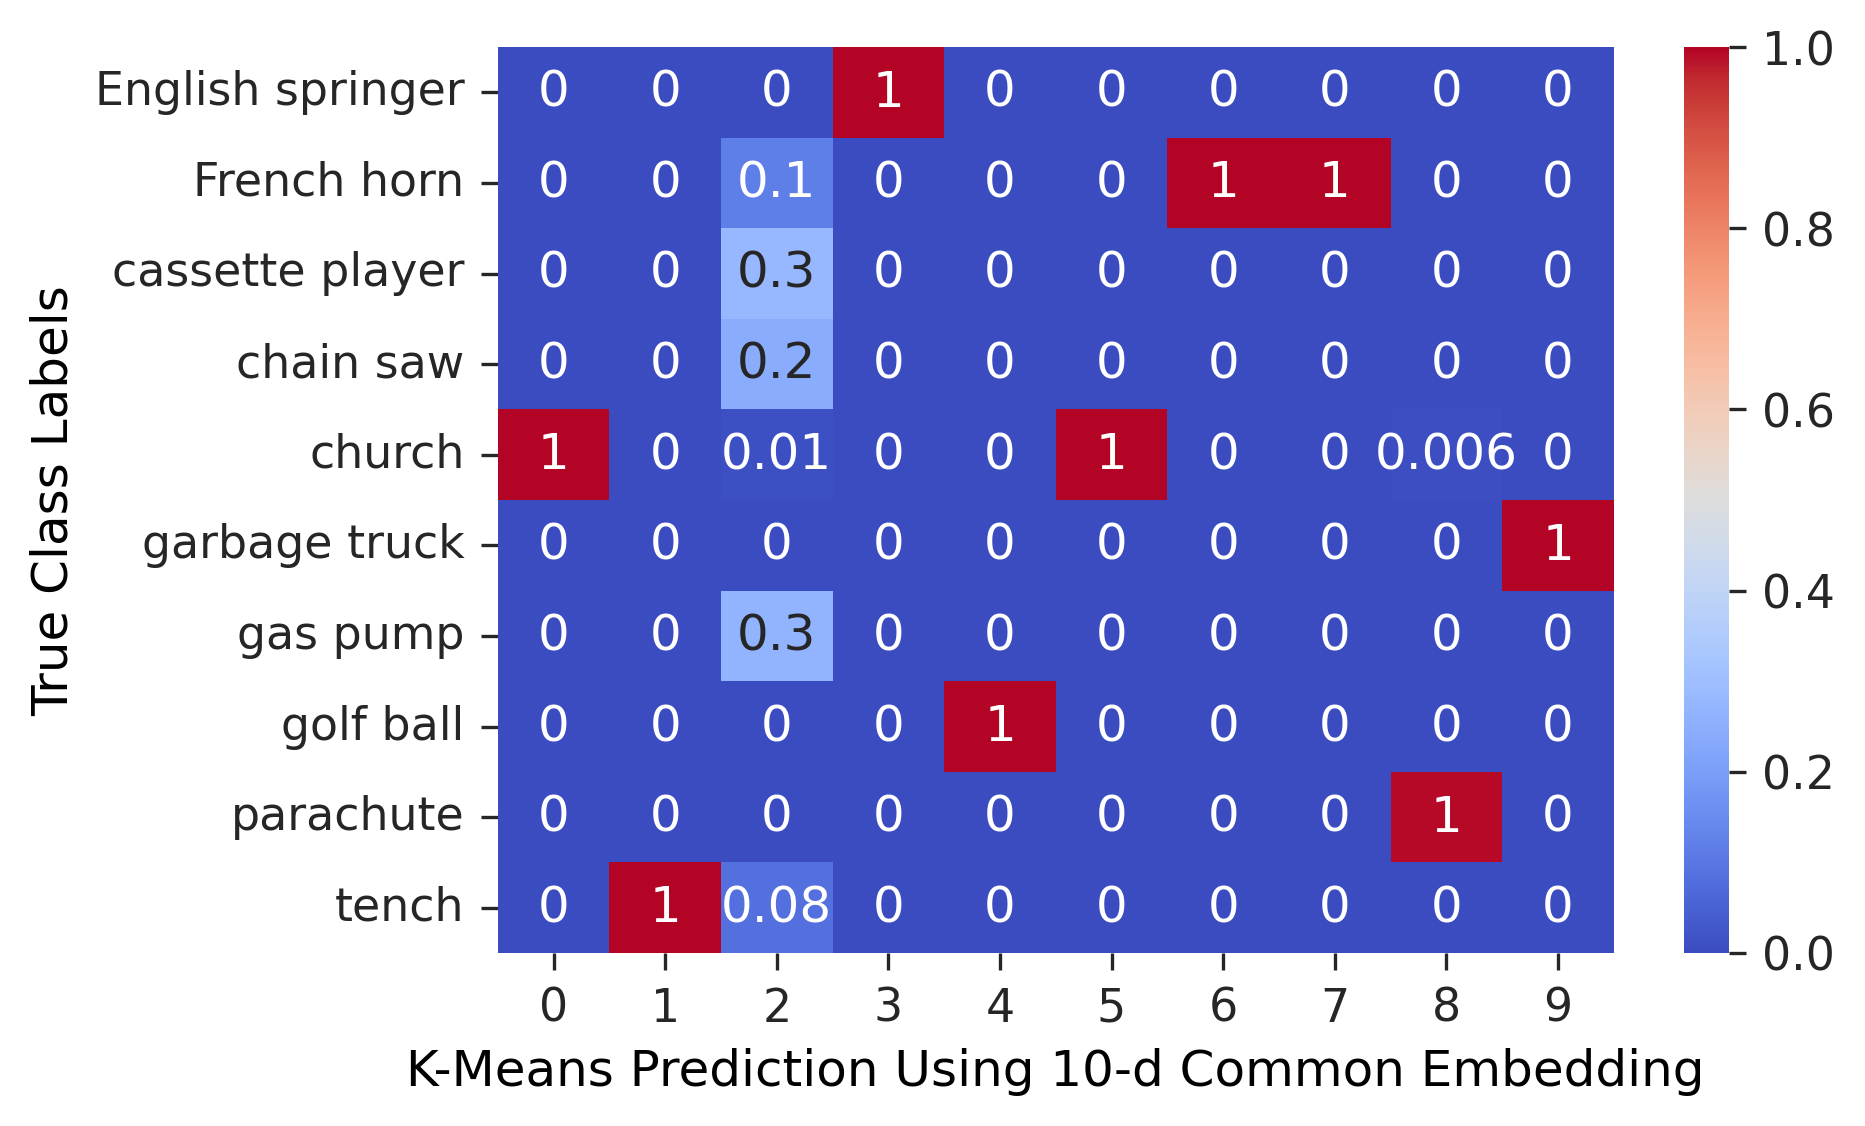
\includegraphics[width=\linewidth]{figure/somefig2.png}
\end{minipage}
\begin{minipage}{0.42\linewidth}
  \centering
  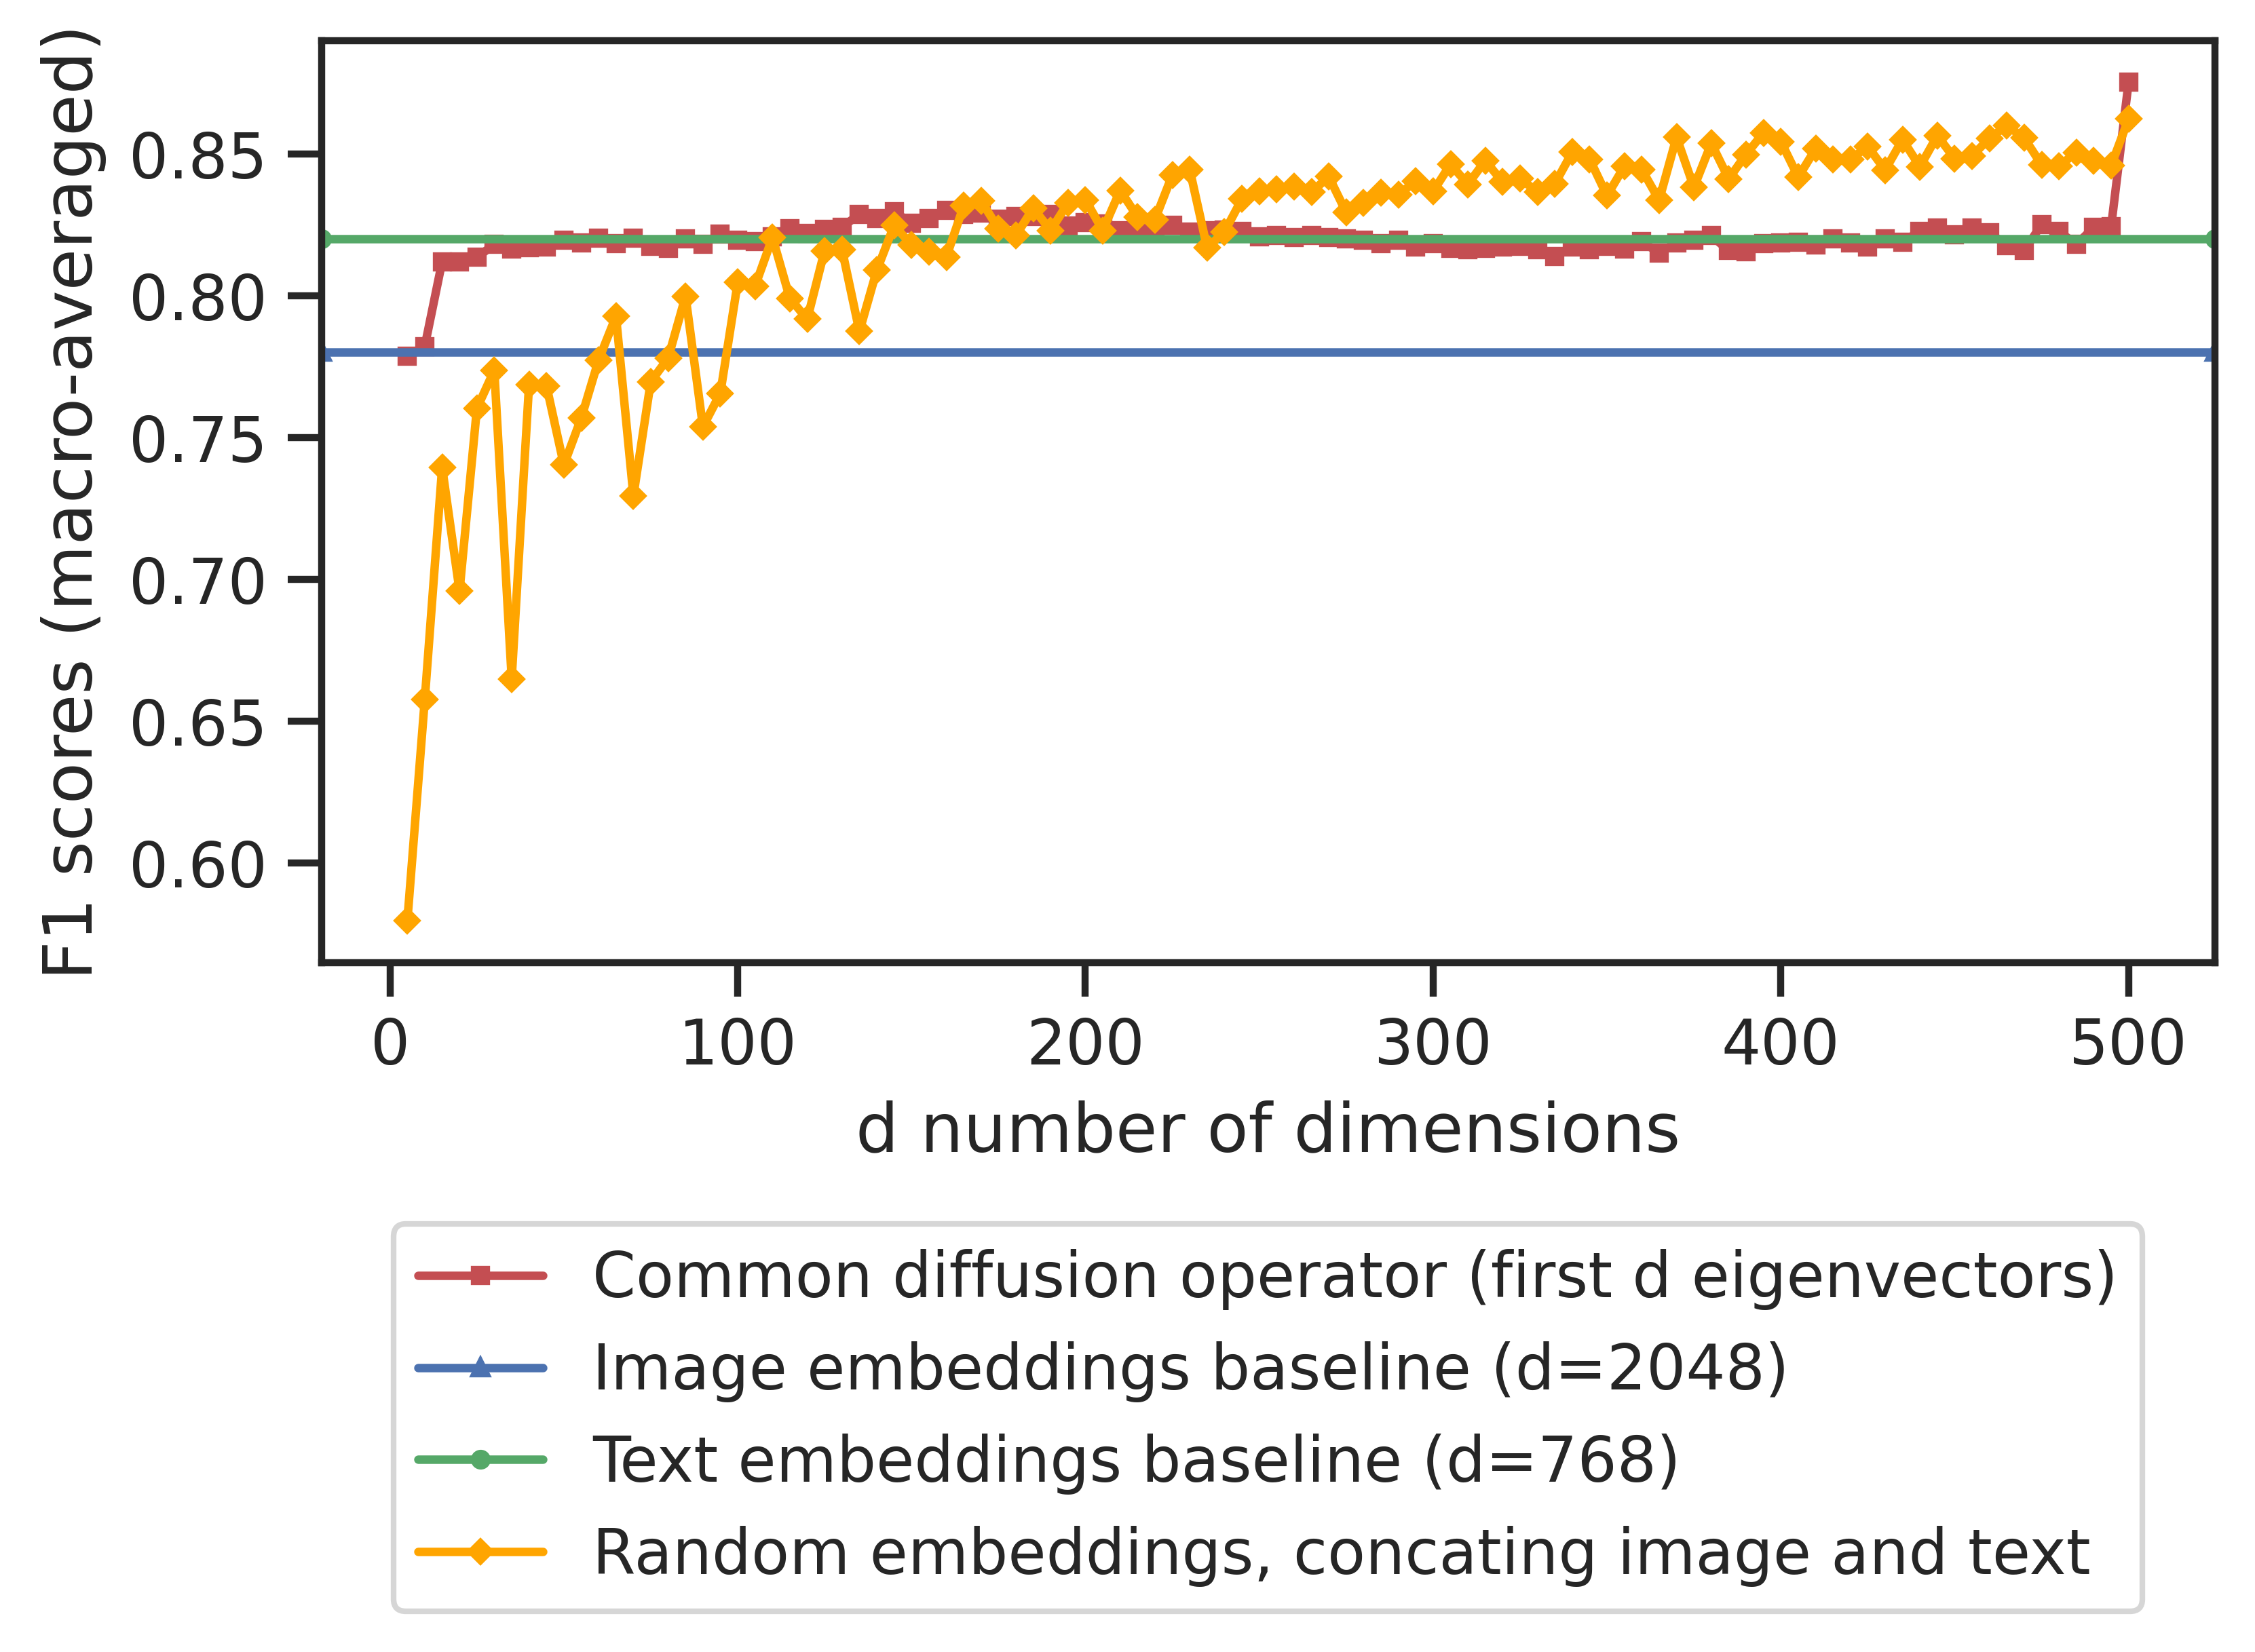
\includegraphics[width=\linewidth]{figure/somefig3.png}
\end{minipage}
\caption{You can put figures side-by-side as well.}
\label{fig:someotherfigs}
\end{figure}


\subsection{Table Examples}

Table \ref{tab:sometab1} presents some summary of the data.

\begin{table}[htbp]
\caption{Some Table Caption}
\label{tab:sometab1}
\resizebox{0.4\linewidth}{!}{\centering
\begin{tabular}{lll}
\toprule
\multicolumn{2}{c}{Part}                   \\
\cmidrule(r){1-2}
Name     & Description     & Size ($\mu$m) \\
\midrule
Dendrite & Input terminal  & $\sim$100     \\
Axon     & Output terminal & $\sim$10      \\
Soma     & Cell body       & up to $10^6$  \\
\bottomrule
\end{tabular}}
\end{table}

Table \ref{tab:sometab2} presents some summaries of the performance of our model.

\begin{table}[htbp]
\caption{Some Other Table Caption}
\label{tab:sometab2}
\resizebox{0.9\linewidth}{!}{\centering
\begin{tabular}{l|lcccccc}
\toprule
Method & Modality & Edit distance & BLEU & METEOR & Precision & Recall & F1 \\ \midrule
PDF                  & All      & 0.255 & 65.8 & 82.1 & 77.1 & 81.4 & 79.2 \\ \hline
GROBID               & All      & 0.312 & 55.6 & 71.9 & 74.0 & 72.1 & 73.0 \\ \cline{2-8}
                     &Tables    & 0.626 & 25.1 & 64.5 & 61.4 & 80.7 & 69.7 \\
+ LaTeX OCR %
                     & Plain text &0.363 & 57.4 & 69.2 & 82.1 & 70.5 & 75.9 \\
                     & Math     & 0.727 & 0.3 & 5.0 & 11.0 & 8.6 & 9.7 \\ \hline
\multirow{4}{*}{Nougat base (350M$^\ast$)} & All & \bf 0.071 & \bf 89.1 & \bf 93.0 & 93.5 & \bf 92.8 & \bf 93.1 \\ \cline{2-8}
                     & Tables     & 0.211 & 69.7 & 79.1 & 75.4 & 80.7 & 78.0 \\ 
                     & Plain text & 0.058         & 91.2 & 94.6   & 96.2      & 95.3   & 95.7 \\
                     & Math       & 0.128         & 56.9 & 75.4   & 76.5      & 76.6   & 76.5 \\ \bottomrule
\end{tabular}}
\end{table}

\subsection{Equations and Algorithms Examples}

Algorithm \ref{alg:fuzzyKmeans} implements Fuzzy K-means.

\begin{algorithm}
\caption{Fuzzy K-means clustering algorithm}
\label{alg:fuzzyKmeans}
\begin{enumerate}
    \item Choose primary centroids $v_{k}$
    \item Compute the membership degree of all feature vectors in all clusters
    \begin{equation}
    u_{ki}  = \frac{1}{ \sum_{j=1}^K ( \frac{D^{2}(x_{i} - v_{k})}{D^{2}(x_{i} - v_{j})})^\frac{2} 
    {m-1}}
    \label{eq:kmeans}
    \end{equation}
\end{enumerate}
\end{algorithm}

Algorithm \ref{alg:net} calculates net activation.


\begin{algorithm}
\caption{Computing Net Activation}
\label{alg:net}
% \DontPrintSemicolon
% \LinesNumbered
\KwIn{$x_1, \ldots, x_n, w_1, \ldots, w_n$}
\KwOut{$y$, the net activation}
$y\leftarrow 0$\;
\For{$i\leftarrow 1$ \KwTo $n$}{
$y \leftarrow y + w_i*x_i$\;
}
\end{algorithm}

In Variational Autoencoder (VAE), we directly maximize the Evidence Lower Bound (ELBO) using the following Equations \ref{eq:bla}--\ref{eq:blablabla}.
\begin{align}
  \mathbb{E}_{q_{\boldsymbol{\phi}}(\boldsymbol{z}\mid\boldsymbol{x})}\left[\log\frac{p(\boldsymbol{x}, \boldsymbol{z})}{q_{\boldsymbol{\phi}}(\boldsymbol{z}\mid\boldsymbol{x})}\right]
  &= \mathbb{E}_{q_{\boldsymbol{\phi}}(\boldsymbol{z}\mid\boldsymbol{x})}\left[\log\frac{p_{\boldsymbol{\theta}}(\boldsymbol{x}\mid\boldsymbol{z})p(\boldsymbol{z})}{q_{\boldsymbol{\phi}}(\boldsymbol{z}\mid\boldsymbol{x})}\right] \label{eq:bla} \\
  &= \mathbb{E}_{q_{\boldsymbol{\phi}}(\boldsymbol{z}\mid\boldsymbol{x})}\left[\log p_{\boldsymbol{\theta}}(\boldsymbol{x}\mid\boldsymbol{z})\right] + \mathbb{E}_{q_{\boldsymbol{\phi}}(\boldsymbol{z}\mid\boldsymbol{x})}\left[\log\frac{p(\boldsymbol{z})}{q_{\boldsymbol{\phi}}(\boldsymbol{z}\mid\boldsymbol{x})}\right] \label{eq:blabla} \\
  &= \underbrace{\mathbb{E}_{q_{\boldsymbol{\phi}}(\boldsymbol{z}\mid\boldsymbol{x})}\left[\log p_{\boldsymbol{\theta}}(\boldsymbol{x}\mid\boldsymbol{z})\right]}_\text{reconstruction term} - \underbrace{\mathcal{D}_{\text{KL}}(q_{\boldsymbol{\phi}}(\boldsymbol{z}\mid\boldsymbol{x}) \mid\mid p(\boldsymbol{z}))}_\text{prior matching term} \label{eq:blablabla}
\end{align}

\subsection{Inline Citation Examples}

Citation in text (no parentheses): use \texttt{{\textbackslash}cite\{citekey\}}. 
For example, \cite{breiman2011}, \cite{devlin2019bert}.

Citation in parentheses: use \texttt{{\textbackslash}citep\{citekey\}}. 
For example: \citep{vaswani2023attention}, \citep{karras2019stylebased}.

\fi


%%%%%%%%%%%%%%%%%%%%%%%%%%%%%%%%%%%%%%%%%%%%%%%%%%%%%%%%
%%%% Reference / Bibliography
%%%%%%%%%%%%%%%%%%%%%%%%%%%%%%%%%%%%%%%%%%%%%%%%%%%%%%%%

\makereference


\bibliography{reference}
\bibliographystyle{style/dsc180bibstyle}

%%%%%%%%%%%%%%%%%%%%%%%%%%%%%%%%%%%%%%%%%%%%%%%%%%%%%%%%
%%%% Appendix
%%%%%%%%%%%%%%%%%%%%%%%%%%%%%%%%%%%%%%%%%%%%%%%%%%%%%%%%

\clearpage
\makeappendix

\subsection{AI Use}
Please refer to the \href{https://github.com/randonDsc/drone_final_project1/blob/main/AI_USE.md}{AI\_USE.md} file for a detailed overview of our AI prompt usage.

%\subsection{Training Details}

%\subsection{Additional Figures}

%\subsection{Additional Tables}


\end{document}